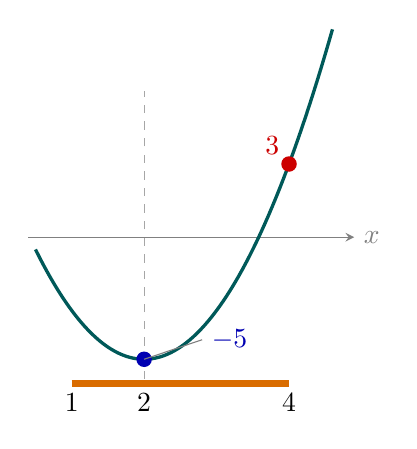
\begin{tikzpicture}[x=0.92cm,y=0.31cm,>=stealth]
 \draw[->,gray] (0.4,0)--(4.9,0) node[right] {$x$};
 \draw[dashed,gray!70] (2,-5.8)--(2,6);
 \draw[very thick,teal!70!black,domain=0.5:4.6,samples=80] plot (\x,{2*(\x-2)^2-5});
 \draw[line width=2.5pt,orange!85!black] (1,-6)--(4,-6);
 \fill[blue!70!black] (2,-5) circle (2.8pt) ;\draw[gray] (2,-5)--(2.8,-4.2) node[right,blue!70!black] {$-5$};
 \fill[red!80!black] (4,3) circle (2.8pt) node[above left] {$3$};
 \node[below] at (1,-6) {$1$}; \node[below] at (2,-6) {$2$}; \node[below] at (4,-6) {$4$};
\end{tikzpicture}
